\chapter{Emulation and Hardware in the loop}
\label{cha:emulation}

The field of emulation is strongly related to the field of simulation and targets the imitation of real world systems.
In contrast to a simulation the purpose of an emulation is to replicate a real world system and providing the possibility to interact with other components in the same way as the emulated system ought to.
Emulation is used in various fields reaching from the replication of outdated computer systems for executing old applications, to the field of \emph{HiL} (hardware in the loop) and the usage for verification and testing of embedded systems. \cite{emulation_koninklijke}

The fields of emulation and \emph{HiL} are based on real-time simulations combined with a connection to the real world.
The replication of a given environment allows to enclose a specific component and then execute specific scenarios.
Such a component can either be a software application (\emph{SiL} - software in the loop) or hardware component (\emph{HiL}).
This connection of simulated systems with real systems can be used for testing and verification of systems under development.
An emulation system running on a host system and an enclosed system under test is shown in figure \ref{fig:emulation_overview}.
The shown structure is typical for various types of emulations with different enclosed systems.

\begin{figure}
\centering
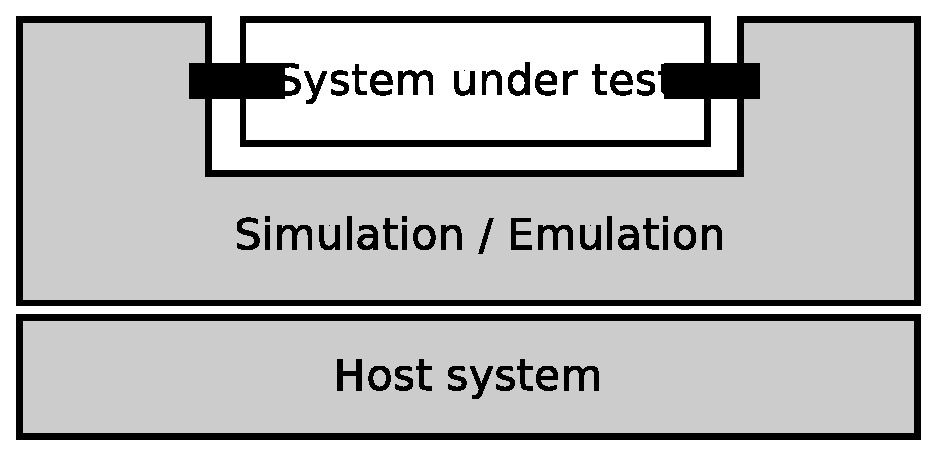
\includegraphics[width=0.7\linewidth]{images/emulation_overview}
\caption{Overview of an emulation environment running on a Host system (gray) with an enclosed system under test (white) and the connections in between those systems (black).}
\label{fig:emulation_overview}
\end{figure}



Such a test method can test various different scenarios due to the flexibility of the simulated system.
\cite[section I]{lu_low-cost_2007}

The used simulation can be realized with any simulation technology and existing simulation frameworks, as long as the execution as real-time simulation (described in section \ref{sec:simulation_real_time}) is possible.
The requirement of real-time simulation must be met for specific given response times to allow the valid interaction with external components.
In the following section the capabilities regarding emulation and \emph{HiL} provided by the OMNeT++ framework are discussed and analyzed.

\section{Emulation and \emph{HiL} using OMNeT++}
\label{sec:emulation_omnet}
For the fields of emulation and \emph{HiL} OMNeT++ provides customizable components within the simulation core and thereby allows different strategies for implementing the required behavior.
The built in functionalities and their usage shown in provided examples are explained in the following section.

\subsection{Existing functionality}
\label{sec:emulation_omnet_existing}

The sample simulation \emph{sockets} shows the possibilities and methods for developing an emulation.
This example simulates a web server with a dynamic number of clients.
For exemplary usage as emulation an external client can also be used, which represents the connection to the real world and communicates with real requests by the user.
These interaction is established via the connection to a local address and the hyper text transfer protocol (\emph{HTTP}) GET request by a web browser.
This emulation uses the custom scheduler \emph{SocketRTScheduler}, which is implemented similar to \emph{cRealTimeScheduler} and derived from \emph{cScheduler}. \cite{omnet_api}
The custom scheduler holds a TCP socket for communication with the real world.
During wait times the schedule listens to the network interface and converts receiving data to simulation events.
These generated events are distributed by the \emph{ExtHttpClient} or \emph{ExtTelnetClient}.
These simple modules represent the external real world components within the simulated network.
The implementation can be found within the \emph{sockets} sample included in the OMNeT++ framework or in the appendix section \ref{app:omnetpp_code_socket}.
This behavior is usable for this exemplary usage, but if the timings of the simulated systems sharpen this scheduler would not allow sufficient communication.
Analyzing the implementation and the achievable timings lead to different possibilities for optimizations as described in \cite{scussel_improvements_2015}.

The combination of a real-time simulation and a real world system requires a connection in between them.
Such a connection can be established using various functionalities, but must always fulfill the functionality of converting occasions form the real world to simulation events and vice versa.
This connection affects the achievable performance and the temporal behavior of the simulated components respectively to the real world component.
In the \emph{sockets} example the built in functionalities for sending and receiving data via sockets are used.
These built in functionalities are implemented depending on the host platform OMNeT++ was built and are therefore using either the \emph{WinSock2} library on Windows operating systems or otherwise the Unix socket implementation.
These built in functionalities for socket communication are located in the \emph{include/platdep} folder within the OMNeT++ installation.
In the following section different strategies and recommendations regarding the communication implementations are discussed.

\section{Communication with the real world}
\label{sec:emulation_communication}
For the fields of emulation and \emph{HiL} the communication with the real world is very important and affects the achievable performance.
By encapsulation of all used communication functionalities in specific modules the simulated model can be clearly separated.
Using OMNeT++ the separated communication components can be realized with modules implementing the connection functionalities or customizing simulation components such as a custom scheduler.
Recommended implementation strategies for each communication functionality and their properties are discussed in the following sections.

\subsection{Receiving}
\label{sec:emulation_communication_receiving}

The receiving component can be implemented as simple module using the \emph{process style} strategy.
This strategy allows an intuitive implementation observing the interface, then creating messages with the received data and sending them to the simulated system.
Executing the simulation sequentially does not allow constant listening by such a receiver module, therefore this must be interrupted to allow the execution of the remaining simulation.
Using parallel simulation described in chapter \ref{cha:parallel_sim} the receiving module can be implemented blocking.
Assigning just the receiving module to a single processor allows a constant listening to the communication interface.
This represents an improved behavior and extended possibility for handling real time occasions and provides a potential lowered delay for the event conversion.

As shown in the \emph{sockets} sample the customization of a simulation component, e.g. the scheduler can also allow the receiving of external data without constantly blocking the simulation.
For this execution method the scheduler \emph{SocketRTScheduler} provides a customized scheduler implementation with a similar strategy as the built in \emph{cRealTimeScheduler}.
This implementation depends strongly on the simulated idle times, because only during these times the reception of data is possible.
Simulating a system with few idle times this strategy can lead to increased delay times until an external occasion is converted to a simulation event.

\subsection{Sending}
\label{sec:emulation_communication_sending}
The sending component can be implemented as simple module either using the \emph{process style} or the \emph{event based} strategy.
Is the sending functionality inevitably blocking this module should be implemented using the \emph{process style} strategy and be executed on a separate processor, when using parallel simulation.
Using a sequential simulation a blocking sending functionality must be used with care to the blocking behavior.
Such behavior could be compensated with timeouts and retries after a defined waiting time while the simulation can proceed.

A similar approach to the receiving implementation using a customized scheduler can also be applied for a non blocking sending.
The prepared data for transmission could be buffered and sent by the scheduler during idle times.
Such buffering affects the timing behavior and must be analyzed regarding achievable response times to external occasions.
\\

For each functionality and depending on the targeted behavior different implementation strategies and design decisions must be made.
Fundamental design strategies regarding the structure of a simulation giving an existing system and their properties are discussed in the next chapter.